\documentclass{beamer}
%
% Choose how your presentation looks.
%
% For more themes, color themes and font themes, see:
% http://deic.uab.es/~iblanes/beamer_gallery/index_by_theme.html
%
\mode<presentation>
{
  \usetheme{Madrid}      % or try Darmstadt, Madrid, Warsaw, ...
  \usecolortheme{seahorse} % or try albatross, beaver, crane, ...
  \usefonttheme{serif}  % or try serif, structurebold, ...
  \setbeamertemplate{navigation symbols}{}
  \setbeamertemplate{caption}[numbered]
} 

\usepackage[english]{babel}
\usepackage{kotex}
\usepackage{tikz}
\usepackage{listings}
\usepackage{pgffor}
\usepackage{listings}
\usepackage{amsfonts}
\usepackage[linesnumbered,ruled,vlined]{algorithm2e}
\usepackage{algorithmic}

% algorithmbis environment
\makeatletter
\newcounter{algorithmbis}[section]
\setcounter{algorithmbis}{0}
\renewcommand{\thealgorithmbis}{\arabic{algorithmbis}}
\def\algorithmbis{\@ifnextchar[{\@algorithmbisa}{\@algorithmbisb}}
\def\@algorithmbisa[#1]{%
  \refstepcounter{algorithmbis}
  \trivlist
  \leftmargin\z@
  \itemindent\z@
  \labelsep\z@
  \item[\colorbox{lightgray}{\parbox{\textwidth}{%
	    \noindent\strut\textbf{\sf\small 코드 \sf\small\thealgorithmbis} \sf\small#1}
  }]\hfil\vskip0em%
  \color{darkgray}
}
\def\@algorithmbisb{\@algorithmbisa[]}
\def\endalgorithmbis{\hfil\endtrivlist}
\makeatother

\lstset{ %
  backgroundcolor=\color{white},   % choose the background color; you must add \usepackage{color} or \usepackage{xcolor}
  basicstyle=\footnotesize,        % the size of the fonts that are used for the code
  breakatwhitespace=false,         % sets if automatic breaks should only happen at whitespace
  breaklines=true,                 % sets automatic line breaking
  captionpos=b,                    % sets the caption-position to bottom
  commentstyle=\color{gray},    % comment style
  deletekeywords={...},            % if you want to delete keywords from the given language
  escapeinside={\%*}{*)},          % if you want to add LaTeX within your code
  extendedchars=true,              % lets you use non-ASCII characters; for 8-bits encodings only, does not work with UTF-8
  frame=single,                    % adds a frame around the code
  keepspaces=true,                 % keeps spaces in text, useful for keeping indentation of code (possibly needs columns=flexible)
  keywordstyle=\color{blue},       % keyword style
  language=C++,                 % the language of the code
  morekeywords={*,...},            % if you want to add more keywords to the set
  numbers=left,                    % where to put the line-numbers; possible values are (none, left, right)
  numbersep=5pt,                   % how far the line-numbers are from the code
  numberstyle=\tiny\color{gray}, % the style that is used for the line-numbers
  rulecolor=\color{black},         % if not set, the frame-color may be changed on line-breaks within not-black text (e.g. comments (green here))
  showspaces=false,                % show spaces everywhere adding particular underscores; it overrides 'showstringspaces'
  showstringspaces=false,          % underline spaces within strings only
  showtabs=false,                  % show tabs within strings adding particular underscores
  stepnumber=1,                    % the step between two line-numbers. If it's 1, each line will be numbered
  stringstyle=\color{gray},     % string literal style
  tabsize=2,                       % sets default tabsize to 2 spaces
  title=\lstname                   % show the filename of files included with \lstinputlisting; also try caption instead of title
}

\title[3D 그래픽스 프로그래밍]{그래픽스 강의노트 06 - 조명 2 (메시)}
\author{강영민}
\institute{동명대학교}
\date{2015년 2학기}

\begin{document}

%%%%%%%%%%%%%%%%%%%%%%%%%%%%%%%%%%%%%%%%%%%%%%%%%%%%%%%%%
\begin{frame}
  \titlepage
\end{frame}

% Uncomment these lines for an automatically generated outline.
%\begin{frame}{Outline}
%  \tableofcontents
%\end{frame}


%%%%%%%%%%%%%%%%%%%%%%%%%%%%%%%%%%%%%%%%%%%%%%%%%%%%%%%%%%
%\begin{frame}[fragile]{깊이 버퍼와 이중 버퍼 사용 예제}
%   \lstset{language=C++,frame=none,escapechar=^}%
%    \foreach \n in {1,26,...,50} {%
%       \only<+>{%
%            \edef\m{\the\numexpr\n+24\relax}%
%            \edef\thesubtitle{{Lines \n--\m\ / 50}}%
%            \expandafter\framesubtitle\thesubtitle
%            \lstinputlisting[firstline=\n,lastline=\m]{./Codes/L03_depthAndDoubleBuffers.tex}%
%       }%
%    }
%\end{frame}
%%%%%%%%%%%%%%%%%%%%%%%%%%%%%%%%%%%%%%%%%%%%%%%%%%%%%%%%%%

%%%%%%%%%%%%%%%%%%%%%%%%%%%%%%%%%%%%%%%%%%%%%%%%%%%%%%%%%
%\begin{frame}[fragile]{간단한 OpenGL 프로그램 테스트}
%\lstset{language=C++,escapechar=^} 
%\begin{lstlisting}
%#include "headers.h"
%
%void myDisplay() {
%   glClear(GL_COLOR_BUFFER_BIT);
%    glFlush();    
%}
%\end{lstlisting}
%\end{frame}
%%%%%%%%%%%%%%%%%%%%%%%%%%%%%%%%%%%%%%%%%%%%%%%%%%%%%%%%%%


%%%%%%%%%%%%%%%%%%%%%%%%%%%%%%%%%%%%%%%%%%%%%%%%%%%%%%%%%
\begin{frame}[fragile]{법선의 설정과 메시(mesh) 데이터 그리기}

앞서 그려본 주전자는 그려지는 면의 법선 벡터가 내장되어 있는 {\sf glutSolidTeapot} 함수를 호출하여 그렸다. 그런데 임의의 면을 그릴 때는 이러한 미리 정의된 법선 벡터가 존재하지 않는다. 그렇다면 퐁 쉐이딩의 계산이 요구되는 법선 벡터는 어떻게 오픈지엘에 넘겨줄 수 있을까?
우선 법선 벡터를 어디에 지정해야 하는지를 생각해 보자. 각각의 정점은 자신의 색을 가져야 하며, 이 색은 퐁 모델을 통해 계산된다. 이때 법선 벡터가 필요하므로 각 정점마다 법선 벡터를 지정해야 한다. 그러면, 각 정점이 아니라 이 정점들이 만드는 다각형의 내부 각 점들은 어떠한가? 각 점들 역시 물체 위의 표면을 나타내며, 각각 색을 결정해야 하므로 법선벡터가 필요하다. 그런데, 일일이 이런 모든 점을 표현하는 픽셀 하나 하나에 법선을 설정하는 것은 거의 불가능하다. 따라서 오픈지엘은 다각형을 구성하는 꼭지점에서의 색을 구한 뒤에 다각형 내부의 색은 이 색들을 보간하여 결정한다.

\end{frame}
%%%%%%%%%%%%%%%%%%%%%%%%%%%%%%%%%%%%%%%%%%%%%%%%%%%%%%%%%

\end{document}



\section{}



그림의 한 면은 세 개의 정점으로 이루어져 있다. 각 정점은 법선 벡터를 가지고 있고, 이 법선 벡터와 조명의 관계를 이용하여 퐁 쉐이딩을 할 수 있다. 그러면 우리는 각 정점의 색을 얻을 수 있다. 그리고 이렇게 얻어진 정점의 색을 이용하여 내부의 특정 픽셀은 선형보간(linear interpolation)을 통해 얻으면 쉽게 내부의 색을 칠할 수 있다. 이러한 내부 색칠 방식을 구로(Gouraud) 쉐이딩이라고 한다. \index{구로 세이딩}\index{Gouraud shading}

\begin{figure}[h!]
  \centering
    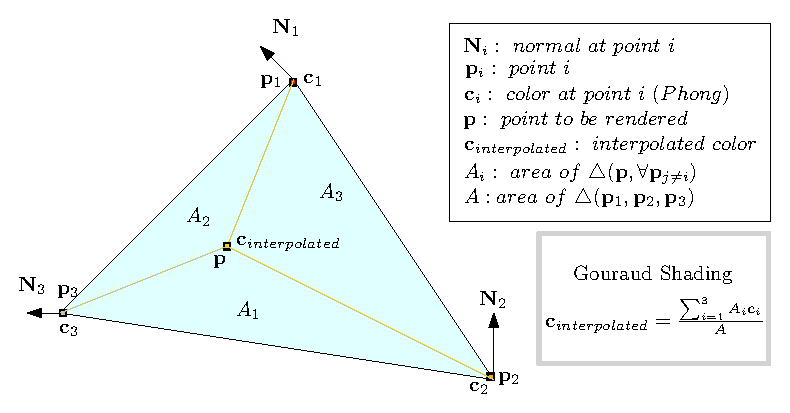
\includegraphics[height=7cm]{OGL_light/interpolatedColors.eps}
    \caption{구로(Gouraud) 세이딩의 계산 방법}
    \label{fig:OGL_light:interpolatedColors}
\end{figure}

구로 세이딩을 할 대상이 그림 \ref{fig:OGL_light:interpolatedColors}와 같이 $\mathbf p_1$, $\mathbf p_2$, $\mathbf p_3$와 같이 세 개의 정점으로 이루어진
삼각형이라고 하자. 각각의 정점에서 가지는 법선 벡터는 $\mathbf N_1$, $\mathbf N_2$, $\mathbf N_3$로 표시하자.
앞에서 살펴본 퐁 모델을 이용하여 각 정점의 색 $\mathbf c_1$, $\mathbf c_2$, $\mathbf c_3$를 계산할 수 있다.
이렇게 계산된 색을 보간하는 것이 구로 세이딩이다. 이때 우리가 색을 칠하려고 하는 대상이 $\mathbf p$라고 하자.
이 지점은 보간된 색상 $\mathbf c_{interpolated}$를 가질 것이다.
이를 계산하기 위해서는 각각의 정점 색깔을 어떤 가중치(weight)로 혼합할 것인지를 결정해야 한다.
삼각형 $\triangle (\mathbf p_1, \mathbf p_2, \mathbf p_3 )$는 정점 $\mathbf p$를 각 정점으로 연결한 선분을 이용하여
그림 \ref{fig:OGL_light:interpolatedColors}처럼 세 구역으로 나뉜다. 하나의 구역은 세 정점 가운데 한 정점 $i$를 뺀 나머지 
두 정점과 그리려는 지점 $\mathbf p$를 연결하여 얻을 수 있고, 이 영역의 넓이를 빠진 정점 $i$의 번호를 달아 $A_i$로 표현하자.
그 이유는 이 영역의 크기가 커지면 $\mathbf p$가 $i$ 지점에 가까워지고, 색도 $\mathbf c_i$에 가까워져야 하기 때문이다.
즉, 이 크기는 색상 $\mathbf c_i$에 곱해지는 가중치로 쓸 수 있다.

구로 세이딩은 보간된 색상 $\mathbf c_{interpoalted}$를 다음과 같이 구한다.

\begin{eqnarray}
\mathbf c_{interpolated} = \frac{\sum_{i=1}^3 A_i \mathbf c_i}{A}
\end{eqnarray}




\begin{figure}[h!]
  \centering
    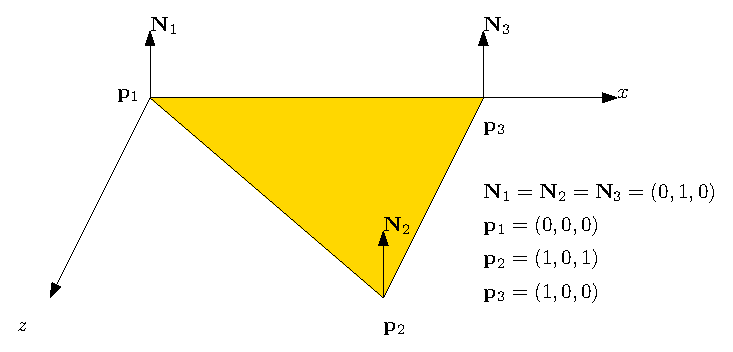
\includegraphics[height=6cm]{OGL_light/simpleTriangle.eps}
    \caption{구로(Gouraud) 세이딩의 계산 방법}
    \label{fig:OGL_light:simpleTriangle}
\end{figure}

이제 간단한 면을 오픈지엘로 렌더링(rendering)해 보자.
간단한 삼각형 하나를 그릴 것이다. 삼각형은 세 개의 정점으로 구성되며, 각 정점은 자기 자신의 정점 좌표를 가진다. 
이 정점 좌표는 이미 {\sf glVertex*} 함수를 통해 지정하는 방법을 사용해 왔다. 이제 각 정점의 법선을 지정하는 방법이 필요하다. 
정점의 법선은 {\sf glNormal*} 함수를 이용하여 설정할 수 있다. 예를 들면 다음 그림 \ref{fig:OGL_light:simpleTriangle}에 나타난 
삼각형을 그린다고 할 때는 아래와 같이 입력한다.

\begin{verbatim}
glNormal3f(0,1,0); glVertex3f(0,0,0);
glNormal3f(0,1,0); glVertex3f(1,1,0);
glNormal3f(0,1,0); glVertex3f(1,0,0);
\end{verbatim}

이제 간단한 면을 그리는 코드 \ref{code:OGL_light:opengl_normalvectors}를  같이 작성해 보자. 이 코드의 실행 결과는 그림 \ref{fig:OGL_light:normalSetting}와 같다. 

\begin{algorithmbis}[삼각형 정점에 법선 부여하기]\label{code:OGL_light:opengl_normalvectors}
\lstset{language=C++} 
\begin{lstlisting}
  glBegin(GL_TRIANGLES);
  glNormal3f(0,1,0);
  glVertex3f(0,0,0);
  glNormal3f(2/sqrt(3),1/sqrt(3),0);
  glVertex3f(2,0,0);
  glNormal3f(-2/sqrt(3),1/sqrt(3),0);
  glVertex3f(1,0,-1);
  glEnd();
\end{lstlisting}
\end{algorithmbis}

\begin{figure}[h!]
  \centering
    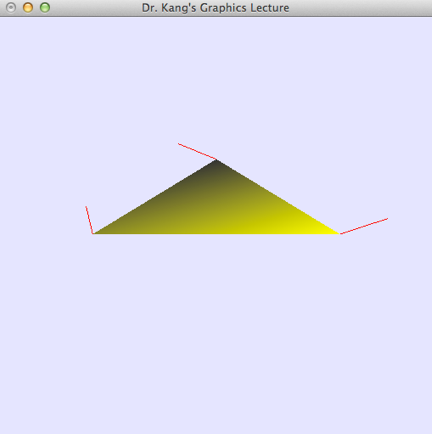
\includegraphics[height=5.5cm]{OGL_light/normalSetting.png}
    \caption{정점별로 법선 벡터를 설정하여 삼각형 그리기 수행 결과}
    \label{fig:OGL_light:normalSetting}
\end{figure}

그림 \ref{fig:OGL_light:normalSetting}의 결과는 코드 \ref{code:OGL_light:opengl_normalvectors}에는 없지만,
설정된 법선벡터를 가시화하기 위한 코드를 추가하여 실행한 결과이며, 각 정점에 설정된 법선 벡터가 선분으로 그려져 있다.
법선벡터가 다르기 때문에 퐁 모델에 의해 각 정점이 서로 다른 색으로 칠해지며,
삼각형 내부는 구로 세이딩을 통해 보간된 색으로 칠해진다.

이제 두 개의 인접한 면을 그려보자. 우선은 각각의 면에 하나씩 법선을 설정하는
코드 \ref{code:OGL_light:twoFacesTwoNormals}와 같이 그려보자. 결과는 그림 \ref{fig:OGL_light:twoFacesTwoNormals}와 같다.

\begin{algorithmbis}[두 개의 면 그리기]\label{code:OGL_light:twoFacesTwoNormals}
\lstset{language=C++} 
\begin{lstlisting}
  glBegin(GL_TRIANGLES);
  glNormal3f(-1/sqrt(2),1/sqrt(2),0);
  glVertex3f(0,1,0);
  glVertex3f(-1,0,0);
  glVertex3f(0,1,1);
  glNormal3f(1/sqrt(2),1/sqrt(2),0);
  glVertex3f(0,1,0);
  glVertex3f(0,1,1);
  glVertex3f(1,0,0);
  glEnd();
\end{lstlisting}
\end{algorithmbis}

\begin{figure}[h!]
  \centering
    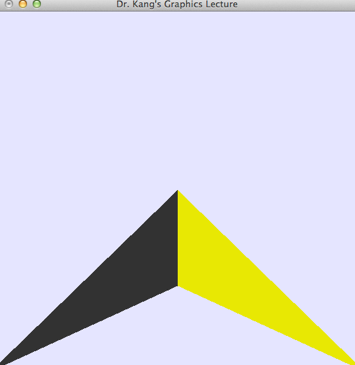
\includegraphics[height=6.0cm]{OGL_light/twoFacesTwoNormals.png}
    \caption{두 개의 면을 서로 다른 두 법선 벡터로 그린 결과}
    \label{fig:OGL_light:twoFacesTwoNormals}
\end{figure}

이렇게 면 별로 서로 다른 법선을 주면 경계가 부드럽게 표현되지 않는다. 이때 두 면에 공유되는 가운데 
두 점은 양쪽 면을 모두 고려하여 (0,1,0)으로 설정하면 다음과 같은 코드 \ref{code:OGL_light:twoFacesFourNormals}처럼 작성할 수 있다.
 실행 결과는 그림 \ref{fig:OGL_light:twoFacesFourNormals}에 보이고 있다.

\begin{algorithmbis}[공유된 점에 공통 법선 부여]\label{code:OGL_light:twoFacesFourNormals}
\lstset{language=C++} 
\begin{lstlisting}
  glBegin(GL_TRIANGLES);
  glNormal3f(0,1,0);  
  glVertex3f(0,1,0);
  glNormal3f(-1/sqrt(2),1/sqrt(2),0);  
  glVertex3f(-1,0,0);
  glNormal3f(0,1,0);  
  glVertex3f(0,1,1);
  glNormal3f(0,1,0);  
  glVertex3f(0,1,0);
  glNormal3f(0,1,0);  
  glVertex3f(0,1,1);
  glNormal3f(1/sqrt(2),1/sqrt(2),0);  
  glVertex3f(1,0,0);
  glEnd();
\end{lstlisting}
\end{algorithmbis}

\begin{figure}[h!]
  \centering
    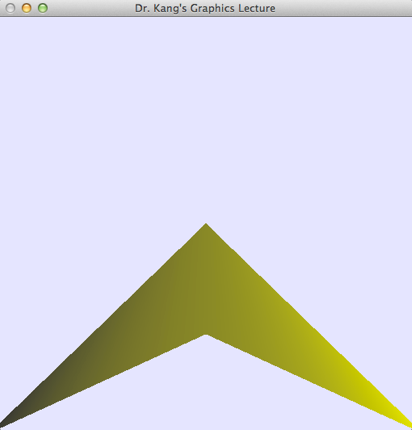
\includegraphics[height=5cm]{OGL_light/twoFacesFourNormals.png}
    \caption{각각의 정점에 서로 다른 법선을 적용}
    \label{fig:OGL_light:twoFacesFourNormals}
\end{figure}

\subsection{메시 읽고 그리기}\index{mesh}\index{메시}

이제 우리는 임의의 메시를 읽고 법선을 계산하여 조명을 비추는 작업을 수행할 것이다.
우선 간단한 메시 데이터 포맷을 정의하자. 
우리의 메시 데이터는 표 \ref{tab:meshDataExample}와 같은 형태를 가진다. 
파일의 가장 처음에 나타나는 것은 전체 정점의 개수 $n$이다. 
그리고 모두 $n$ 개의 정점에 대해 위치 정보가 3차원 벡터로 나타난다.
그 다음은 면의 개수 $m$이 온다. 그리고 이어지는 정보는
$m$ 개의 면이 가진 정점 정보를 보여준다.
하나의 면은 삼각형으로 이루어지고, 면을 표현하는 정보는 이 삼각형을 구성하는
정점의 번호 세 개가 나타난다.
하나의 정점은 1에서 $n$ 사이의 정수 하나로 표현할 수 있다. 
오른쪽 칼럼의 내용은 우리가 앞서 그려본 도형을 메시 파일로 표현한 것이다.


\begin{table}
\caption{메시 데이터 포맷의 예시}
\label{tab:meshDataExample}
\begin{center}
    \begin{tabular}{ |l|l|}
    \hline
    {\small \sf 포맷} & {\small \sf 실제 데이터 예시} \\ \hline
\pbox{10cm}{\small \sf numVertices $n$\\ vertex 1 ($x_1,y_1,z_1$)\\ vertex 2 ($x_2,y_2,z_2$)\\ ...\\ vertex $n$ ($x_n,y_n,z_n$)\\ numFaces $m$\\ face 1 ($f_1.v_1,f_1.v_2,f_1.v_3$)\\ face 2 ($f_2.v_1,f_2.v_2,f_2.v_3$)\\ ...\\ face m ($f_m.v_1,f_m.v_2,f_m.v_3$)} & 
\pbox{10cm}{\small \sf 4\\ 0.0 1.0  0.0\\ -1.0  0.0  0.0\\  0.0  1.0  1.0\\  1.0  0.0  0.0\\ 2\\ 0 1 2\\  0 2 3 } \\ 
\hline
\end{tabular}
\end{center}
\end{table}

이러한 메쉬를 읽어 들이는 클래스를 작성해 보자. 우선 헤더 파일에서 클래스의 기본적인 설계를 해 보자. 다음 코드 \ref{code:OGL_light:meshClass}와 같은 구조가 될 것이다.
이 메쉬 클래스는 {\sf cvertex}라는 정점 데이터를 저장하는 클래스와, 면 데이터를 저장하는 {\sf cface} 클래스를 먼저 정의한다. 정점은 3차원 좌표이다. 면은 세 개의 정점으로 구성되는데, 정점의 좌표나 정점 객체를 그대로 쓰는 것이 아니라 정점이 저장된 배열의 색인(index)로 표현한다. 
메쉬 클래스에서 가장 중요한 데이터는 정점 데이터이다. 메쉬 전체를 이루는 정점의 개수와 면의 개수가 멤버 변수로 있고, 정점은 {\sf cvertex} 형 배열로 다뤄진다. 면은 {\sf cface} 형 배열이다. 추가로 사용되는 데이터는 메쉬를 읽고 나서 전체적인 크기를 파악할 수 있는 바운딩 박스 정보이다. 축정렬(axis-aligned) 바운딩 박스를 사용하여 {\sf minx, miny, minz, maxx, maxy, maxz}의 값으로 표현된다. 외부 인터페이스로는 생성자와 함께, 메쉬를 읽는 {\sf loadMesh}, 메쉬를 그리는 {\sf drawMesh} 두 함수만 있다.


\begin{algorithmbis}[메시 클래스 정의]\label{code:OGL_light:meshClass}
\lstset{language=C++, escapechar=^} 
\begin{lstlisting}
#ifndef _mesh_sms_hh_
#define _mesh_sms_hh_
class cvertex {
public:
    float x;
    float y;
    float z;
}; // ^{\it 하나의 점을 구성하는 좌표값 3 개}^
class cface {
public:
    int v0; int v1; int v2;
}; //^{\it 하나의 삼각형 면을 구성하는 세 개 정점의 인덱스들}^

class CMesh {
    int nV;  // ^{\it 정점의 개수}^
    int nF;  // ^{\it 메시 구성 삼각형 면의 수}^
    cvertex *v; // ^{\it 정점 데이터 배열}^
    cface   *f; // ^{\it 면 데이터 배열}^

public:
    float minx, miny, minz;
    float maxx, maxy, maxz; // ^{\it 메시를 둘러싸는 AABB 경계상자}^

public:
    CMesh();  // constructor
    ~CMesh(); // destructor
    // ^{\it 메시를 읽고 그리는 메소드들}^
    void loadMesh(char *meshFileName);
    void drawMesh(void);
};
#endif
\end{lstlisting}
\end{algorithmbis}

이제 {\sf mesh.cpp} 파일을 작성할 것이다. 우선 생성자와 메쉬를 읽어들이는 코드를 작성해 보자. 생성자는 정점와 면의 개수를 0으로 설정하고, 정점과 면 데이터를 저장할 배열을 {\sf NULL}로 설정한다. 또한 바운딩 박스 데이터에서 {\sf min} 값을 매우 큰 음수로, {\sf max}는 매우 큰 값으로 설정해 둔다.

메쉬 파일을 읽어 들이는 {\sf loadMesh} 역시 매우 간단하다. 파일을 열고, 처음으로 정점의 개수를 {\sf nV}로 읽어 들인다. 
그리고 이 {\sf nV} 개수 만큼의 배열을 생성한 뒤에 차례로 좌표를 읽어 저장한다. 이때 좌표를 보고 {\sf min, max} 값들을 변경한다. 
다음으로 면의 개수를 읽어 들여 {\sf nF}에 저장하고, {\sf nF} 개의 면에 대해 각각 세 개 씩의 정점 색인을 읽어 저장한다.
코드 \ref{code:OGL_light:meshImplementation}와 같이 구현이 가능하다.

\begin{algorithmbis}[메시 클래스 구현]\label{code:OGL_light:meshImplementation}
\lstset{language=C++,escapechar=^} 
\begin{lstlisting}
#include "Mesh.h" 

^{\sf [[필요한 헤더 파일들 포함]]}^

#define BIGNUMBER 100000000000000000000000.0

CMesh::CMesh() : nV(0), nF(0), v(NULL), f(NULL),
    minx( BIGNUMBER), miny( BIGNUMBER), minz( BIGNUMBER),
    maxx(-BIGNUMBER), maxy(-BIGNUMBER), maxz(-BIGNUMBER) { }

CMesh::~CMesh() {
    if(v) delete[] v;
    if(f) delete[] f;    
}

void CMesh::loadMesh(char *meshFileName) {
    FILE *fptr = fopen(meshFileName, "r");
    if(!meshFileName || !fptr) {     
       printf("file open error\n"); exit(0);    
    }

    // ^{\it 정점의 개수 읽기}^
    fscanf(fptr, "%d", &nV);
    v = new cvertex[nV];
    for (int i=0; i<nV; i++) {
        // ^{\it {\sf nV}개의 정점 정보를 읽음}^
        fscanf(fptr, "%f", &v[i].x); 
        fscanf(fptr, "%f", &v[i].y); 
        fscanf(fptr, "%f", &v[i].z);
    }

    // ^{\it 면의 개수 읽기}^
    fscanf(fptr, "%d", &nF);
    f = new cface[nF];
    for (int i=0; i<nF; i++) {
        // ^{\it {\sf nF}개의 면 정보를 읽음}^
        fscanf(fptr, "%d", &f[i].v0);   
        fscanf(fptr, "%d", &f[i].v1);    
        fscanf(fptr, "%d", &f[i].v2);
    }
}
\end{lstlisting}
\end{algorithmbis}

그림을 그리는 {\sf drawMesh}는 다양한 방법으로 구현이 가능하다. 우선 읽어 들인 정점을 그대로 화면에 찍어 보는 다음과 같이
메시를 구성하는 정점을 출력하는 코드 \ref{code:OGL_light:meshVertexDraw}를 작성해 보자.


\begin{algorithmbis}[정점 화면 출력]\label{code:OGL_light:meshVertexDraw}
\lstset{language=C++} 
\begin{lstlisting}
void CMesh::drawMesh(void) {
  if(!v || !f) return;
  glBegin(GL_POINTS);
  for(int i=0;i<nV;i++) {
    glVertex3f( v[i].x, v[i].y, v[i].z);
  }
  glEnd();
}
\end{lstlisting}
\end{algorithmbis}

이 코드 \ref{code:OGL_light:meshVertexDraw}를 실행하면 
그림 \ref{fig:OGL_light:drawMeshVerts}와 같은 결과를 얻을 수 있다.

\begin{figure}[h!]
  \centering
    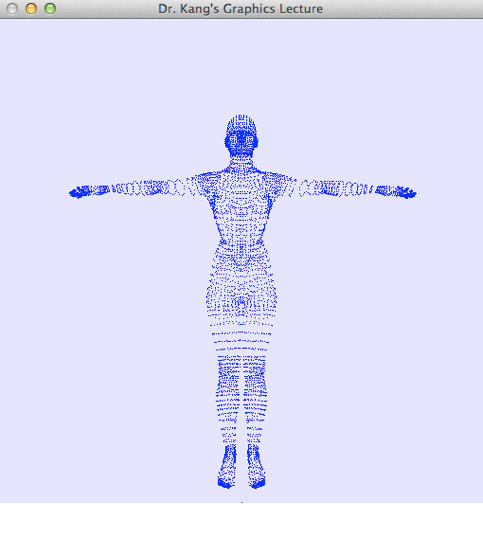
\includegraphics[height=6cm]{OGL_light/drawMeshVerts.png}
    \caption{메시의 정점을 그린 결과}
    \label{fig:OGL_light:drawMeshVerts}
\end{figure}

메쉬의 drawMesh 함수를 변경하여 각 면을 그리도록 코드를 코드 \ref{code:OGL_light:meshEdgeDraw}와 같이 변경해 보자.

\begin{algorithmbis}[메시의 간선을 그리기]\label{code:OGL_light:meshEdgeDraw}
\lstset{language=C++, escapechar=^} 
\begin{lstlisting}
void CMesh::drawMesh(void) {
    for (int i=0; i<nF; i++) {
        // ^{\it i-번째 면을 그리는 작업}^
        int a, b, c; // ^{\it 삼각형을 구성하는 세 정점의 인덱스}^
        a = f[i].v0; // ^{\it i-번째 면의 0번 정점}^
        b = f[i].v1; // ^{\it i-번째 면의 1번 정점}^
        c = f[i].v2; // ^{\it i-번째 면의 2번 정점}^
        glBegin(GL_LINE_LOOP);
        glVertex3f(v[a].x, v[a].y, v[a].z); // ^{\it a 정점의 좌표}^
        glVertex3f(v[b].x, v[b].y, v[b].z);// ^{\it b정점의 좌표}^
        glVertex3f(v[c].x, v[c].y, v[c].z); // ^{\it c 정점의 좌표}^
        glEnd();
    }
}
\end{lstlisting}
\end{algorithmbis}

이 코드는 점이 아니라 면을 그리며, 각 면이 가진 세 개의 색인을 이용하여 정점 배열에서 좌표를 얻어온다. 
결과는 그림 \ref{fig:OGL_light:meshEdgeDraw}와 같다.

\begin{figure}[h!]
  \centering
    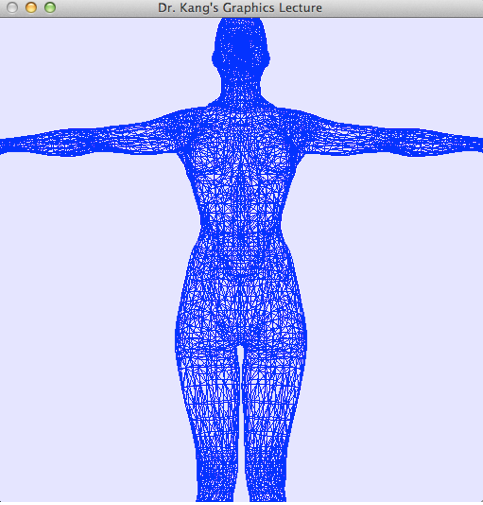
\includegraphics[height=10cm]{OGL_light/meshEdgeDraw.png}
    \caption{메시의 간선(edge)들을 그린 결과}
    \label{fig:OGL_light:meshEdgeDraw}
\end{figure}

다음으로 이 메쉬를 와이어프레임(wireframe) 구조가 아니라 채워진 면을 그리고자 한다. 면을 그릴 때에는 각 면이 조명을 받아 어떤 색상과 밝기를 갖는지가 결정되어야 한다. 조명 설정은 앞의 절에서 살펴본 방식대로 하면 될 것이다. 이 조명 환경에서 각각의 면들이 가진 밝기를 계산하기 위해서는 법선 벡터가 필요하다. 어떤 면의 법선 벡터를 구하는 것은 그 면 위의 서로 다른 두 벡터를 구해 외적한 뒤 정규화하면 된다.

하나의 삼각형에는 세 개의 정점이 있고, 한 정점에서 다른 어떤 정점의 좌표를 빼면 평면 위에 있는 벡터가 된다. 따라서 좌표가 주어진 삼각형 정점 세 개에서 두 개의 벡터를 구하는 것은 매우 간단한 일이다. 이 두 벡터를 외적하여 법선을 구할 수 있다. 

각각의 면을 그리면서 {\sf GL\_TRIANGLES} 프리미티브를 이용하여 채워진 면이 그려지도록 하며, 
이때 각 점의 법선은 앞서 설명한 방법으로 계산하여 그리도록 하는 코드는 다음의 코드 \ref{code:OGL_light:meshFlatSurfaces}와 같다.

\begin{algorithmbis}[법선을 계산하여 메시의 면을 그리기]\label{code:OGL_light:meshFlatSurfaces}
\lstset{language=C++, escapechar=^} 
\begin{lstlisting}
void CMesh::drawMesh(void) {

    if(!v || !f) return;
    glBegin (GL_TRIANGLES) ; 

    for(int i=0;i<nF;i++) {

        // ^{\it 법선 벡터를 계산하기 위한 정보}^
        cvertex p0, p1, p2;  // ^{\it 세 개의 정점 ${\mathbf p}_0, {\mathbf p}_1, {\mathbf p}_2$}^
        cvertex v0, v1; cvertex n; //^{\it 면 위의 두 벡터 ${\mathbf v}_0, {\mathbf v}_1$와 법선벡터 $\mathbf n$}^
        p0 = v[f[i].v0];
        p1 = v[f[i].v1];
        p2 = v[f[i].v2];

        // ^{\it ${\mathbf v}_0 = {\mathbf p}_1 - {\mathbf p}_0$}^
        v0.x = p1.x-p0.x; v0.y = p1.y-p0.y; v0.z = p1.z-p0.z; 
        // ^{\it ${\mathbf v}_1 = {\mathbf p}_2 - {\mathbf p}_0$}^
        v1.x = p2.x-p0.x; v1.y = p2.y-p0.y; v1.z = p2.z-p0.z;

        // ^{\it ${\mathbf n} = \frac{{\mathbf v}_1 \times {\mathbf v}_0}{|{\mathbf v}_1 \times {\mathbf v}_0|}$}^
        n.x = v0.y*v1.z-v0.z*v1.y;
        n.y = v0.z*v1.x-v0.x*v1.z;
        n.z = v0.x*v1.y-v0.y*v1.x;
        float len = sqrt(n.x*n.x+n.y*n.y+n.z*n.z); 
        n.x /= len; n.y /= len; n.z /= len;

        glNormal3f(n.x, n.y, n.z); 
        glVertex3f( p0.x, p0.y, p0.z); 
        glVertex3f( p1.x, p1.y, p1.z); 
        glVertex3f( p2.x, p2.y, p2.z);
    }
    glEnd() ;

}
\end{lstlisting}
\end{algorithmbis}

이 코드 \ref{code:OGL_light:meshFlatSurfaces}를 실행한 결과가
그림 \ref{fig:OGL_light:meshFlatSurfaces}에 나타나 있다.

\begin{figure}[h!]
  \centering
    \fbox{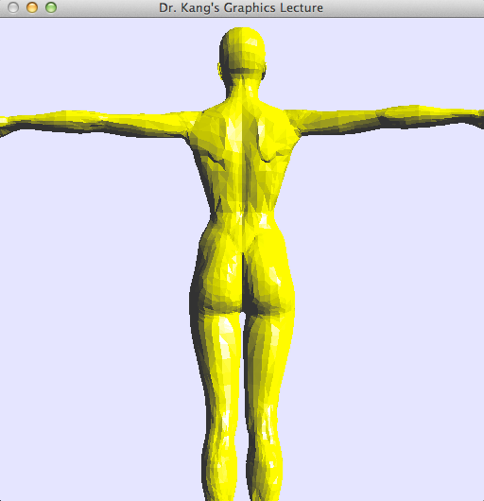
\includegraphics[height=10cm]{OGL_light/meshFlatSurfaces.png}}
    \caption{메시의 면을 그린 결과 (면 단위로 법선 계산)}
    \label{fig:OGL_light:meshFlatSurfaces}
\end{figure}

이 코드의 문제점은 무엇일까? 우선 매번 면을 그릴 때마다 법선벡터를 계산하는 것은 비효율적이다. 따라서 메쉬가 만들어지면 한 번 법선 벡터를 계산한 뒤, 이 결과를 각 정점별로 저장해 두는 것이 좋다. 그런데, 앞의 코드는 동일한 정점이라도 서로 다른 면에 사용될 때는 서로 다른 법선을 갖게 된다. 그렇기 때문에 위의 그림과 같은 면별 쉐이딩이 이뤄진다. 
이런 문제를 해결하기 위해서는 정점 별로 법선벡터를 계산해야 하며, 어떤 정점의 법선 벡터는 그 정점을 포함하는 모든 면들의 법선을 
함께 고려해야 한다. 이때 필요한 법선 벡터의 수는 정점의 수와 동일하며, 3차원 벡터가 된다.

이러한 점을 고려하여 {\sf CMesh} 클래스를 수정할 필요가 있다. 
수정의 내용은 코드 \ref{code:OGL_light:meshClassFinal}에서 볼 수 있는 것처럼 정점 정보와 같은 형(type)과 크기의 배열 {\sf n}을 준비하는 것과
필요할 때에만 법선 벡터 계산을 할 수 있도록 법선 벡터 계산을 명시적으로 호출할 수 있는 메소드
{\sf computeNormals()}를 선언하는 것이다.

\begin{algorithmbis}[정점 별로 법선을 저장하기 위한 배열 추가]\label{code:OGL_light:meshClassFinal}
\lstset{language=C++, escapechar=^} 
\begin{lstlisting}
class CMesh {
    int nV;  // number of vertices
    int nF;  // number of faces
    cvertex *v; // vertex array
    cface   *f; // face array
    cvertex *n; // ^{\it \color{red} 법선 벡터의 배열}^
...
public:
...
    void computeNormals(void); // ^{\it \color{red} 법선 벡터를 계산하여 {\sf n}에 채움}^
};

#endif
\end{lstlisting}
\end{algorithmbis}

법선 벡터의 배열 {\sf n}에 필요한 메모리 공간을 동적으로 할당하는 일은
메시 데이터를 읽어 들일 때에 이루어진다.
그리고, 법선 벡터를 계산하는 작업을 구현하는 것은 코드 \ref{code:OGL_light:meshClassImplementation}과 같은
방식으로 할 수 있다.

{\sf loadMesh} 메소드의 마지막에 읽어들인 정점의 수 {\sf nV}를 이용하여 동적 배열 할당을 수행하고,
입력된 데이터를 이용하여 법선 벡터를 계산하는 {\sf computeNormals} 메소드를 호출한다.
이 {\sf computeNormals} 메소드는 앞에서 법선 벡터를 계산했던 방식과 동일한 방법으로
각각의 면에 대해 법선 {\sf N}을 계산한다. 그런데, 이 법선 벡터는 바로 사용되지 않는다.
어떤 면을 구성하는 정점이 $\mathbf p_0, \mathbf p_1, \mathbf p_2$라면
각각의 법선 벡터를 $\mathbf n_0, \mathbf n_1, \mathbf n_2$라고 할 수 있다.
계산된 법선 벡터 {\sf N}은 이들에게 각각 더해져서 누적된다.
\begin{eqnarray}
\mathbf n_0 = \mathbf n_0 + N \\ \nonumber
\mathbf n_1 = \mathbf n_1 + N \\ \nonumber
\mathbf n_2 = \mathbf n_2 + N \\ \nonumber
\end{eqnarray}
그리고 나서, 모든 $\mathbf n_i$에 대해 정규화를 수행하면 각 정정별 법선을 얻을 수 있다.

\begin{algorithmbis}[법선 벡터 배열의 생성과 법선 벡터 계산의 구현]\label{code:OGL_light:meshClassImplementation}
\lstset{language=C++, escapechar=^} 
\begin{lstlisting}
void CMesh::loadMesh(char *meshFileName) {

    ^{\sf [[앞 부분은 이전 코드와 동일]]}^
    
    ^{\bf \color{red}n = new cvertex[nV]; // {\it \color{black}법선 벡터 배열에 메모리 공간을 할당}}^
    ^{\bf \color{red}computeNormals();}^
    
}

void CMesh::computeNormals(void) { // private method
    
    for(int i=0;i<nV;i++) {
        n[i].x = n[i].y = n[i].z = 0.0;
    }
    
    for(int i=0; i<nF; i++) {
        // ^{\it 각각의 면에 대해서 외적을 이용한 법선 계산을 수행한다}^
        cvertex p0, p1, p2;
        cvertex v0, v1; cvertex N;
        int vert0, vert1, vert2;
        vert0 = f[i].v0; vert1 = f[i].v1; vert2 = f[i].v2;
        p0 = v[vert0];
        p1 = v[vert1];
        p2 = v[vert2];
        v0.x = p1.x-p0.x; v0.y = p1.y-p0.y; v0.z = p1.z-p0.z;
        v1.x = p2.x-p0.x; v1.y = p2.y-p0.y; v1.z = p2.z-p0.z;
        
        N.x = v0.y*v1.z-v0.z*v1.y;
        N.y = v0.z*v1.x-v0.x*v1.z;
        N.z = v0.x*v1.y-v0.y*v1.x;

        // ^{\it 이렇게 얻어진 법선 벡터는 이 면을 구성하고 있는 정점 3 개의 법선 데이터에 누적된다}^
        n[vert0].x += N.x; n[vert0].y += N.y; n[vert0].z += N.z;
        n[vert1].x += N.x; n[vert1].y += N.y; n[vert1].z += N.z;
        n[vert2].x += N.x; n[vert2].y += N.y; n[vert2].z += N.z;
    }
    
    for(int i=0;i<nV;i++) {
        // ^{\it 모든 정정에 대해 누적된 법선 벡터를 정규화한다}^
        float len = sqrt(n[i].x*n[i].x+n[i].y*n[i].y+n[i].z*n[i].z);
        n[i].x /= len; n[i].y /= len; n[i].z /= len;
    }
    
}
\end{lstlisting}
\end{algorithmbis}

이제 우리는 그림 \ref{fig:OGL_light:meshSmoothSurfaces}와 같이 부드러운 면을 가진 메시를 그릴 수 있게 되었다.

\begin{figure}[h!]
  \centering
    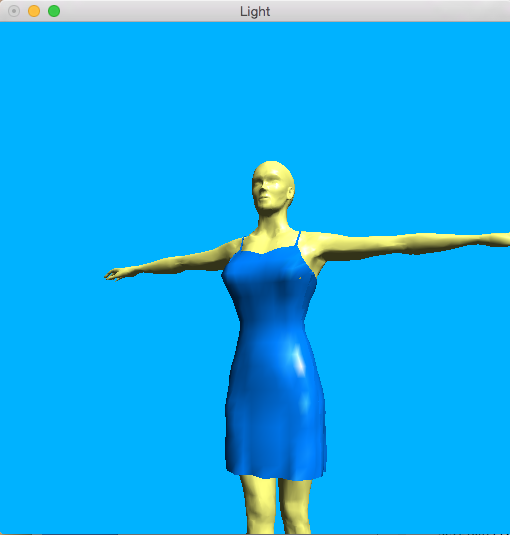
\includegraphics[height=10cm]{OGL_light/meshSmoothSurfaces.png}
    \caption{메시의 면을 그린 결과 (정점 단위로 법선 계산)}
    \label{fig:OGL_light:meshSmoothSurfaces}
\end{figure}
